\bookchapter{Capítulo 60: Preparando o ambiente de desenvolvimento — Xcode e o primeiro projeto}

\chapterintro{Para fazer bem feito, comece pelas ferramentas. Neste capítulo vamos montar a “cozinha”: instalar o Xcode, rodar o simulador, criar o primeiro projeto iOS da sua vida e entender a estrutura do projeto em detalhes. Com o ambiente pronto, você vai ver pela primeira vez o seu código virar um botão que responde ao toque — um momento que muita gente guarda para sempre.}

\booksection{Prepare um Mac}

Começando pela exigência: desenvolver para iOS precisa ser feito no macOS. Se você não tem um Mac, há três saídas: comprar um (até um Mac mini ou MacBook Air usado serve), alugar um Mac na nuvem por um tempo ou começar pela oitava parte, “Prática de desenvolvimento Android” (que dá para fazer no Windows).

\begin{center}
\begin{tabularx}{\linewidth}{|X|X|X|}
\hline
\textbf{Item} & \textbf{Mínimo} & \textbf{Confortável (recomendado)} \tabularnewline
\hline
Chip & Apple Silicon (a partir do M1) & M2 ou mais novo \tabularnewline
Memória & 8GB & 16GB \tabularnewline
Disco & Reserve 40 GB ou mais (o Xcode é bem gordinho) & A partir de 256 GB \tabularnewline
Sistema & macOS mais recente & Mantenha a atualização automática \tabularnewline
\hline
\end{tabularx}
\end{center}

\begin{center}\small\color{gray}Referência de configuração de um Mac para desenvolvimento (agosto de 2026)\end{center}

\begin{tcbinfo}{Dica: dá para aprender a linguagem antes de ter um Mac}
O Swift Playgrounds, gratuito no iPad, ensina o básico da linguagem Swift (sem precisar de Mac); dá até para instalar no iPhone. Aprenda bem o conteúdo do Capítulo 61 brincando no Playgrounds e, quando chegar o Mac, você decola. Afiar o machado não atrasa o corte — é exatamente disso que se trata.

\end{tcbinfo}

\booksection{Instale o Xcode}

O Xcode é o ambiente de desenvolvimento integrado oficial da Apple, e é gratuito. Instalação em três passos:

\begin{enumerate}
  \item No Mac, abra a App Store, busque “Xcode” e clique em instalar — atenção, ele tem vários GB, então escolha um horário com boa conexão;
  \item Ao abrir pela primeira vez depois da instalação, aceite o acordo e deixe os componentes terminarem de baixar (é automático);
  \item No menu Xcode > Settings > Locations, confira se o Command Line Tools está selecionado — as ferramentas de linha de comando são pré-requisito de muitos scripts e ferramentas de terceiros.
\end{enumerate}

\begin{tcbwarn}{Atenção: o “jogo de encaixe” entre versões e sistema}
O Xcode novo costuma exigir o macOS mais recente, e Macs antigos ficam presos em versões antigas. Para publicar na App Store, a Apple pede builds feitos com um Xcode relativamente novo (geralmente com um período de tolerância). Por isso, não demore para atualizar o sistema — desenvolvedores iOS estão entre os que mais correm atrás das versões novas.

\end{tcbwarn}

\booksection{Crie seu primeiro projeto}

Abra o Xcode > Create New Project > escolha iOS > modelo App e preencha:

\begin{center}
\begin{tabularx}{\linewidth}{|X|X|X|}
\hline
\textbf{Item} & \textbf{O que preencher} & \textbf{Explicação} \tabularnewline
\hline
Product Name & MyFirstApp & Nome do app \tabularnewline
Team & Seu Apple ID (gratuito) & Para a assinatura; conta pessoal serve \tabularnewline
Organization Identifier & com.example & Forma o identificador do pacote junto com o Product Name \tabularnewline
Interface & SwiftUI & Framework principal deste livro \tabularnewline
Language & Swift & Fala por si \tabularnewline
\hline
\end{tabularx}
\end{center}

\begin{center}\small\color{gray}As cinco coisas a preencher ao criar o projeto\end{center}

Depois de clicar em Create, o Xcode gera um projeto pronto para rodar. No canto superior esquerdo, escolha um simulador (por exemplo, iPhone 17) e clique no > para executar — em poucos segundos, uma janela com “Hello, world!” aparece na tela do simulador. Seu primeiro app iOS acabou de nascer.

\booksection{Anatomia do projeto: para que serve cada arquivo}

À esquerda fica o navegador do projeto; para começar, você só precisa conhecer estes:

\begin{center}
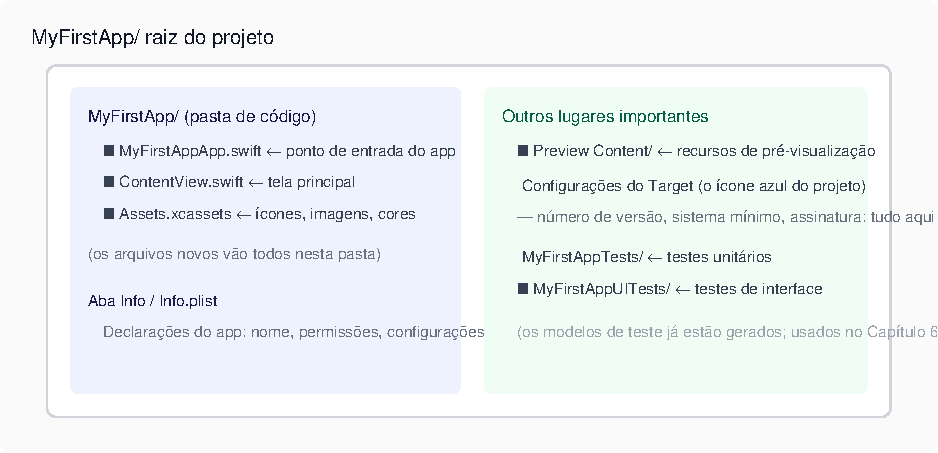
\includegraphics[width=0.92\linewidth]{figures/fig-di-liu-shi-zhang-1}
\\[2pt]\small Figura 2: a estrutura de projeto do Xcode que todo iniciante precisa conhecer
\end{center}

\begin{itemize}
  \item MyFirstAppApp.swift: o ponto de entrada do programa; no SwiftUI ele tem só algumas linhas — “inicie e mostre a tela principal”;
  \item ContentView.swift: a view da tela principal; tudo o que você vê agora está aqui;
  \item Assets.xcassets: o depósito de recursos — ícones, imagens e cores ficam aqui;
  \item Configurações do Target: clique no ícone azul do projeto à esquerda para entrar; número da versão, versão mínima do iOS e assinatura ficam aí. O nome de exibição e o ícone do app também se configuram nesse lugar.
\end{itemize}

\booksection{Testes no aparelho: colocando o app no seu iPhone}

\booksection{Truques de eficiência no Xcode: os cinco “cheats de atalhos” do iniciante}

Dominando estes, você vai parecer “bem profissional”:

\begin{center}
\begin{tabularx}{\linewidth}{|X|X|X|}
\hline
\textbf{Ação} & \textbf{Atalho} & \textbf{Função} \tabularnewline
\hline
Executar & CmdR & Compila e roda o app \tabularnewline
Abrir/alternar a pré-visualização do canvas & OptionCmd & O interruptor do “o que você vê é o que você tem” \tabularnewline
Formatar a indentação & CtrlI & Organiza automaticamente a indentação do código selecionado \tabularnewline
Abrir arquivo rapidamente & CmdO & Digite o nome do arquivo e ele abre na hora (o mais usado!) \tabularnewline
Comentar/descomentar & Cmd/ & Ligar e desligar trechos de código durante o debug \tabularnewline
\hline
\end{tabularx}
\end{center}

\begin{center}\small\color{gray}Atalhos mais usados do Xcode (o kit do iniciante)\end{center}

Mais dois benefícios escondidos: rodar vários simuladores ao mesmo tempo (iPhone e iPad lado a lado para comparar layouts) e a biblioteca de snippets de código (arraste as linhas que você usa sempre para o painel de Snippets à direita e insira com um clique na próxima vez) — use as ferramentas de eficiência desde cedo e a fluidez vem naturalmente.

\booksection{Testes no aparelho: colocando o app no seu iPhone}

O simulador é ótimo, mas o aparelho de verdade é o destino final. Dá para testar no aparelho até com um Apple ID gratuito:

\begin{enumerate}
  \item Conecte o iPhone pelo cabo de dados (ou faça o debug sem fio no mesmo Wi-Fi);
  \item Na lista de aparelhos no topo do Xcode, selecione seu celular; na primeira vez, ele pedirá para entrar com o Apple ID e configurará a assinatura automaticamente;
  \item No iPhone, vá em [Ajustes] > [Geral] > [VPN e Gerenciamento de Dispositivos] e confie no seu certificado de desenvolvedor;
  \item Clique no > e o app é instalado no aparelho.
\end{enumerate}

\begin{tcbwarn}{Atenção: a “regra dos sete dias” da conta gratuita}
Um app assinado com Apple ID gratuito expira depois de 7 dias (basta rodar de novo uma vez para renovar). É um mecanismo da Apple contra abuso e, na fase de aprendizado, dá e sobra; a conta de desenvolvedor paga (99 dólares/ano) não tem essa limitação — detalhes no Capítulo 67.

\end{tcbwarn}

\booksection{Um primeiro teste + primeiros socorros para erros comuns}

\booksection{Um primeiro teste + primeiros socorros para erros comuns}

Abra o ContentView.swift, troque o texto de Text(“Hello, world!”) pelo seu nome e pressione CmdR para rodar de novo — em poucos segundos, seu nome aparece no simulador. Parabéns: você acabou de completar o primeiro ciclo completo de “editar código > compilar > instalar > executar”.

\begin{center}
\begin{tabularx}{\linewidth}{|X|X|X|}
\hline
\textbf{Sintoma do erro} & \textbf{Causa comum} & \textbf{Solução} \tabularnewline
\hline
Erro de Signing & Team não selecionado ou certificado vencido & Em Target > Signing, marque sua conta; com conta gratuita, rode de novo uma vez \tabularnewline
Simulador com tela preta / não abre & Imagem corrompida & Menu Device > Erase All Content; ou apague o simulador e crie outro \tabularnewline
Xcode baixa devagar / não instala & Instabilidade de rede na App Store & Troque de horário; ou baixe o pacote .xip no site de desenvolvedores da Apple \tabularnewline
\hline
\end{tabularx}
\end{center}

\begin{center}\small\color{gray}Tabela de primeiros socorros para erros de ambiente de iniciantes\end{center}

\begin{tcbpractice}{Mãos à obra: complete sua lista de “ritual de desenvolvedor”}
(1) Instale o Xcode e faça o simulador funcionar; (2) rode seu app no aparelho de verdade e tire uma captura de tela para guardar; (3) troque o texto de Hello pelo seu nome; (4) nas configurações do Target, mude o nome de exibição do app para “Meu primeiro app”. Com esses quatro passos feitos, você já é alguém com uma obra própria.

\end{tcbpractice}

\begin{tcbsummary}{Resumo do capítulo}
\begin{itemize}
  \item Exigências: Mac + Xcode; sem Mac, aprenda a linguagem primeiro no Swift Playgrounds do iPad
  \item Instale o Xcode pela App Store; versões novas exigem sistema novo — não adie a atualização
  \item Os cinco pontos ao criar um projeto: nome, Team, identificador da organização, SwiftUI e Swift
  \item Regra de bolso do projeto: o código fica todo na pasta MyFirstApp/; as configurações do Target cuidam de versão e assinatura
  \item Com Apple ID gratuito, o debug no aparelho tem limite de 7 dias de assinatura; a conta paga não tem essa limitação
  \item A rotina de desenvolvimento = editar código > CmdR > ver o resultado, em ciclo contínuo
\end{itemize}

\end{tcbsummary}
